\documentclass[11pt, a4paper]{article}
\usepackage[utf8]{inputenc}
\usepackage[colorlinks=true,linkcolor=blue,urlcolor=blue]{hyperref}
\usepackage{graphicx}
\graphicspath{{images/}}

\begin{document}
    \title{%
	Android Doze impacts on 802.11 power saving \\
	\large Wireless Internet 091034\\
	Prof. Redondi\\
	2017/2018}

    \author{Stefano Brandoli 875633\\Silvia Calcaterra 874887}
    \date{\today}

	\maketitle
	\begin{center}
	    
\includegraphics[scale=0.3]{Logo_Politecnico_Milano.png}
	\end{center}
	\newpage
	\tableofcontents
	\newpage
	
	\section{Motivations}
	With the announcement of Android Marshmallow (Android M 6.0), Google introduced a new power saving functionality called \href{https://android.hdblog.it/2015/06/02/android-m-funzionamento-di-doze/}{Doze}, aiming to intelligently prolongue the lifetime of Android smartphones, tablets and wearable devices.
	
	The survey here presented aims to investigate what is the real impact on 802.11 power saving functionalities for devices where Doze is enabled.
	
	\section{Testing environment}
	\subsection{Smartphone}
	We've always used the same device, an \href{https://www.gsmarena.com/lg_nexus_5-5705.php}{LG Nexus 5 (LG-D821)}, so that our results have not been influenced by different hardware. The system images for the LG Nexus 5 can be found \href{https://developers.google.com/android/images#hammerhead}{here}. The Nexus 5 has been flashed twice using \href{https://developers.google.com/android/images#instructions}{fastboot} and these very different images:
	\begin{itemize}
		\item \textbf{Android KitKat 4.4.4 (KTU84P): no Doze}
		\item \textbf{Android M 6.0.1 (M4B30Z): with Doze}
	\end{itemize}

	In most of the cases the Nexus 5 system images contain also an updated version of the Baseband. The Baseband is the firmware that controls all radio devices on the phone, including GPS, WiFi, Bluetooth, NFC, cellular data and voice. Because these functions are highly regulated and certified, they are separated from the main operating system. In our experiments we've always flashed \href{https://www.androidpit.com/how-to-update-nexus-5-bootloader-and-radio}{the same Baseband} (latest version: M8974A-2.0.50.2.30), so that our results have not been influenced by different 802.11 low level firmwares.
	
	\begin{figure}[h]
        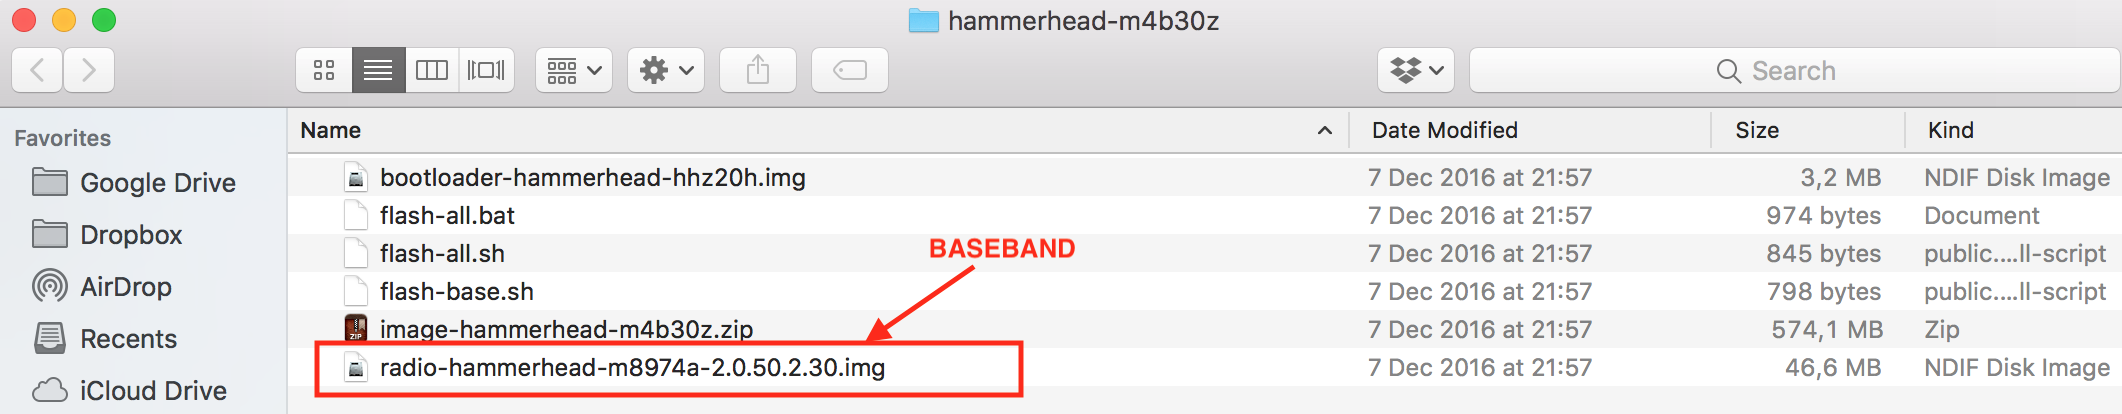
\includegraphics[width=\textwidth]{baseband.png}
        \centering
    \end{figure}

	The Nexus 5 mounts a \href{https://www.ifixit.com/Teardown/Nexus+5+Teardown/19016#s53729}{Broadcom BCM4339 wireless card}, which includes on-chip 2.4 and 5 GHz transmit power amplifiers and receive low noise amplifiers. It supports up to 802.11ac.
	
	\subsection{Access Point}
	The access point used in our experiments is the \href{https://www.asus.com/it/Networking/DSLN55U_Annex_A/}{ASUS DSL-N55U}.
	It supports up to 802.11n and it's dual-channel (2.4 GHz and 5 GHz). Further specifications can be found \href{https://www.asus.com/it/Networking/DSLN55U_Annex_A/specifications/}{here}. The \href{https://www.asus.com/it/Networking/DSLN55U_Annex_A/HelpDesk_BIOS/}{latest available firmware} has been flashed. It is used to set up a BSS.
	
	\subsection{Computer}
	A Macbook Pro Retina (A1502) 13 inch Early 2015 has been used for capturing packets. This pc mounts a \href{https://www.ifixit.com/Store/Mac/MacBook-Pro-13-Inch-Retina-Early-2015-Airport-Bluetooth-Board/IF123-048-1}{wireless card} able to work on both 2.4 GHz and 5 GHz, supporting up to 802.11ac.
	
	\subsection{Software Tools}
	\begin{itemize}
		\item \textbf{Wireshark 2.4.5}: powerful tool to capture packets
		\item \textbf{Python 3.6}: data analysis using \textbf{pyshark} and \textbf{matplotlib.pyplot}.
	\end{itemize}

	\section{Experiment Setup}
	\subsection{Applications Considered}
	In our experiments with Android KitKat and Android M we've setup the exact same configuration of Android applications, namely:
	\begin{itemize}
	    \item \textbf{Chat}: Telegram and WhatsApp
	    \item \textbf{Email}: Gmail: 3 accounts (2 personal, 1 POLIMI account)
	    \item \textbf{Social}: Facebook and Facebook Messenger
	    \item \textbf{Free time}: YouTube, Google Keep, Maps, Photos, Chrome, News and Weather, News, Play Store
	\end{itemize}
	
	\noindent In addition:
	\begin{itemize}
	    \item The rest of the stock applications have been uninstalled, disabled or never used
	    \item The backup of application's data with Google servers has been enabled
	    \item Push notifications have been enabled on all the applications which use them
	    \item "Optimize Battery" (needed by Doze) has been enabled for each application
	\end{itemize}
	
	\subsection{Doze and Aggressive Doze}
	In the Android OS applications holding \textbf{wakelocks} are one of the main causes of abnormal power consumption. While the device is asleep with the screen off, a wakelock allows an Android application to wake up temporarily the device to perform some activity (network, notifications, background services, etc\dots). The request of a wakelock may however prevent the device from going into a power-saving deep sleep mode. To put limits on the abuse of wakelocks by Android applications (which actually don't always need them), Android 6.0 Marshmallow introduced Doze.
	
	On Android 6 Marshmallow \href{https://lifehacker.com/how-android-doze-works-and-how-to-tweak-it-to-save-you-1785921957}{Doze is activated} if your phone’s screen is off, if it’s not charging and if the phone has been stationary for some hours. In this state, all wakelocks are blocked, network access is disabled, jobs/syncs and alarms are deferred and \textbf{no GPS or WiFi scans are performed until a maintenance window}. The next image, taken from \href{https://www.xda-developers.com/how-android-n-will-improve-battery-and-memory-management/}{XDA developers}, further clarifies:
	
	\begin{figure}[h]
        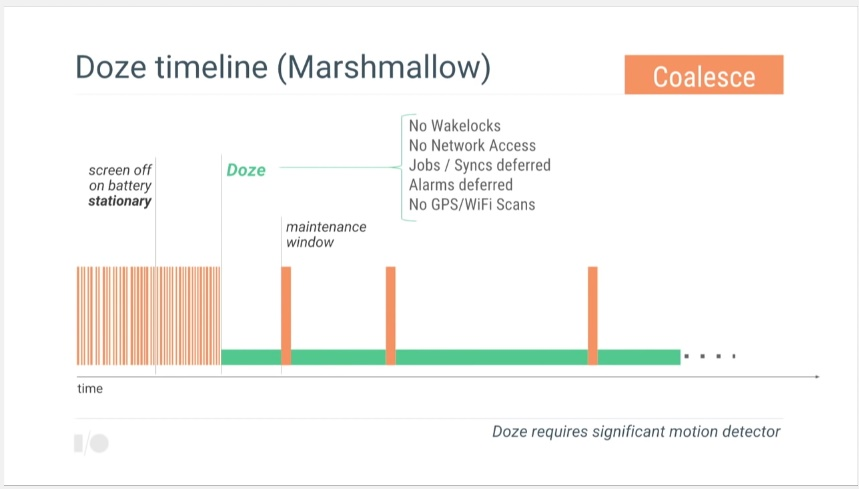
\includegraphics[width=0.9\textwidth]{dozeandroid6}
        \centering
    \end{figure}

	Some applications, like \href{https://play.google.com/store/apps/details?id=com.oasisfeng.greenify&hl=it}{Greenify}, allow to \textbf{enable Doze after some minutes of inactivity (instead of some hours)} with a feature called \href{https://greenify.uservoice.com/knowledgebase/articles/828360-what-is-aggressive-doze}{Aggressive Doze}. We've decided to activate this advanced option and to allow Greenify to show debug notifications (when the device screen was turned on) relative to the Dozing periods. With Aggressive Doze, Doze has always triggered after some minutes of inactivity as expected.
	
	\begin{figure}[h]
        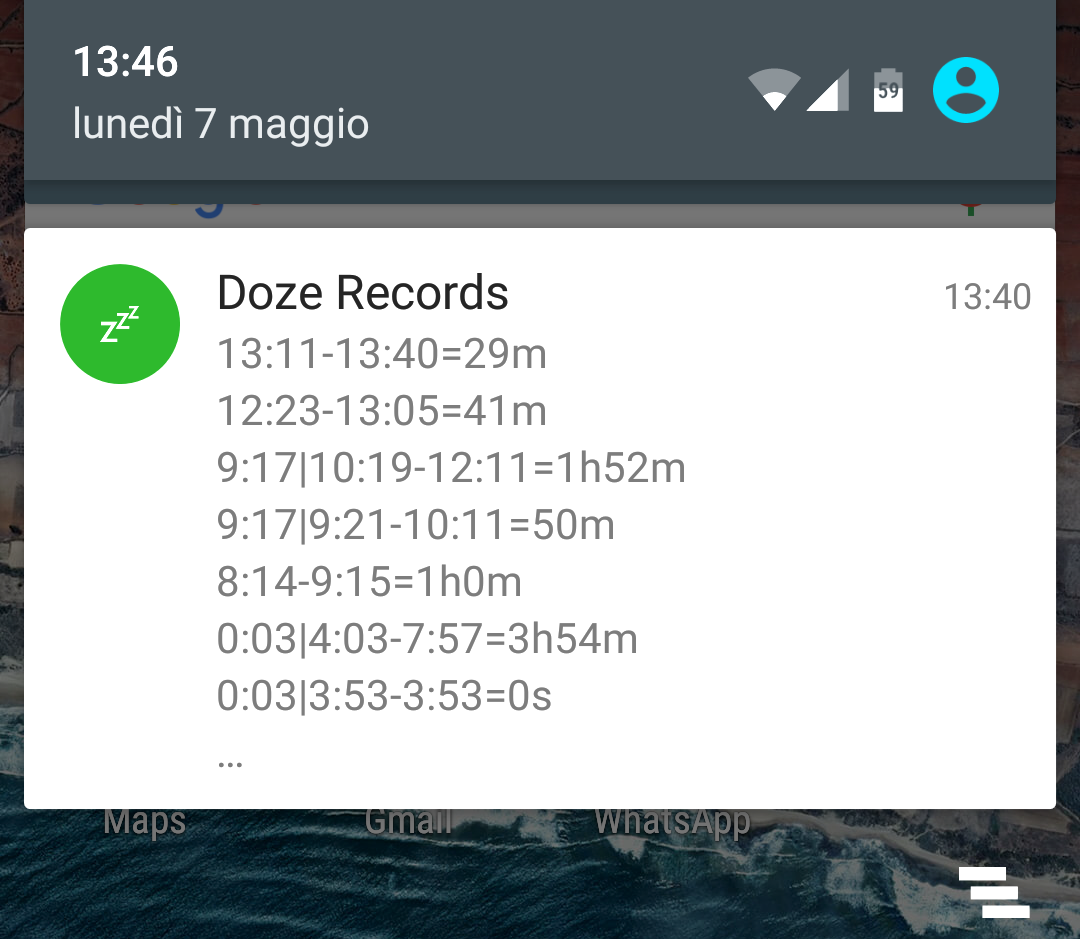
\includegraphics[width=7cm]{dozeRecs.png}
        \centering
    \end{figure}
	
	\subsection{Capturing packets}
	We've decided to capture packets in \textbf{2 scenarios}:
	\begin{itemize}
	    \item 2.4 GHz
	    \item 5 GHz
	\end{itemize}
	Aggressive Doze has allowed us to compare, even on short captures, the full benefits of Dozing (Android 6) vs no Dozing (Android 4.4.4) and its effects on 802.11 power saving functionalities. Thus we've decided to perform \textbf{captures of these durations}:
	   \begin{itemize}
	       \item 10 minutes
	       \item 30 minutes
	       \item 1 hour
	       \item 2 hours
	       \item 3 hours
	   \end{itemize}
	 In particular:
	 \begin{itemize}
	     \item For each capture we've used on Wireshark the \textbf{Capture Filter wlan host Nexus5MAC}, to capture only packets sent/received by our Nexus 5.
	     \item The Nexus 5's screen hasn't been turned on nor the device recharged for the whole time of a capture.
	     \item For each scenario and capture's duration we've performed more than 5 tests in total, during different days and different clock's hours.
	     \item We have not considered captures lower than 10 minutes because in our experiments, even with Aggressive Doze, the device has never gone Dozing for that durations.
	     \item 5 GHz captures have been performed with the Nexus 5 very close to the AP (1 meter) to try to limit packets' retransmissions.
	 \end{itemize}
	    
	\newpage
	\section{Results}
	The following results, both on 2.4 GHz and 5 GHz, consider only the packets that our Nexus 5 has sent to the access point in different capture durations. 
	
	\subsection{2.4 GHz}
	    
        \begin{figure}[ht]
           \centerline{
             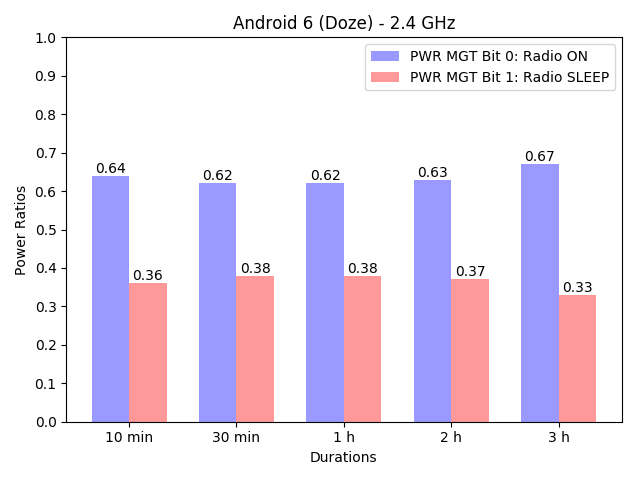
\includegraphics[width=8cm]{00_doze6_pwr_2_4.png}
             \hfill
             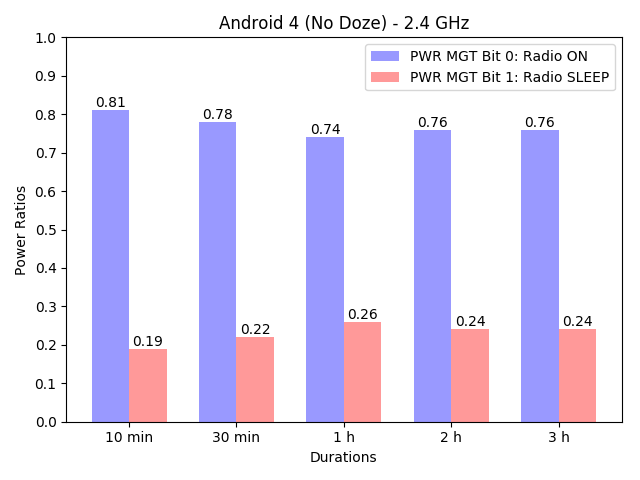
\includegraphics[width=8cm]{01_nodoze4_pwr_2_4.png}
           }
        \end{figure}

        \begin{figure}[ht]
          \centerline{
            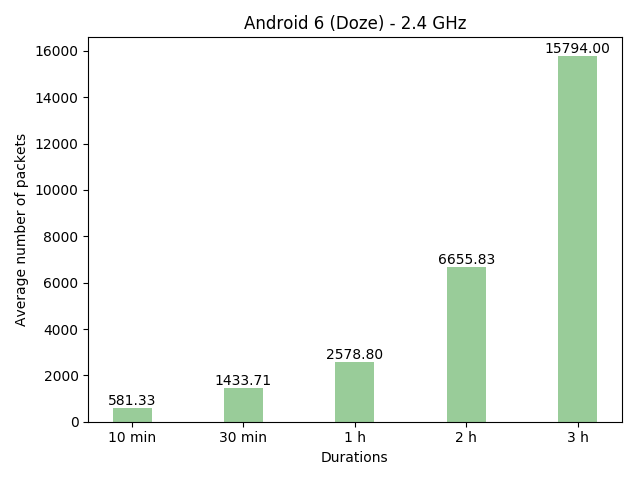
\includegraphics[width=8cm]{02_doze6_avg_pkt_2_4.png}
            \hfill
            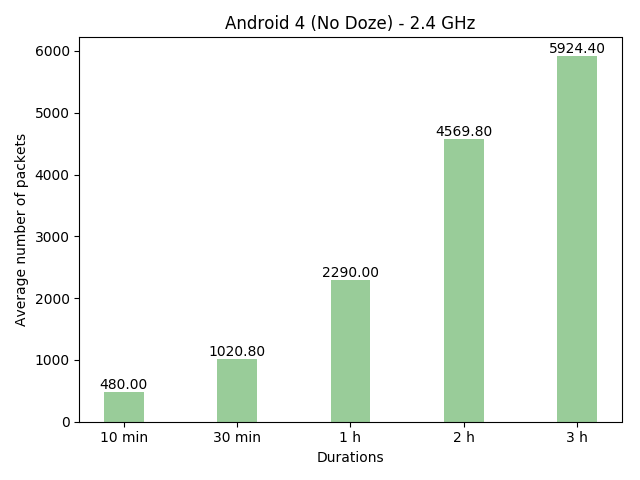
\includegraphics[width=8cm]{03_nodoze4_avg_pkt_2_4.png}
           }
        \end{figure}
        
        Considering all the capture durations, the usage of Doze on Android 6 appears to have significantly increased the number of times when the PWR MGT bit = 1 wrt Android 4, which implies that the 802.11 radio is sleeping more and thus saving more energy.
        
        On Android 6, the power ratios appear to be more or less constant (PWR MGT bit = 1 $\simeq{0.3}$, PWR MGT bit = 0 $\simeq{0.6}$) despite the capture duration. This means that more or less 1/3 of the time the 802.11 radio is sleeping and also that Doze is immediately effective even on short time durations.
        
        Also on Android 4 the power ratios appear to be more or less constant (PWR MGT bit = 1 $\simeq{0.2}$, PWR MGT bit = 0 $\simeq{0.8}$) despite the capture duration, but they are "less stable" wrt to what happens on Android 6. 
        
        In this case the 802.11 radio is sleeping more or less 1/5 of the time, leading to a less energy efficient behaviour wrt the one of Android 6.

        We've decided to compute the average number of packets sent, expecting it to be lower on Android 6 wrt Android 4, since Doze defers WiFi scans. Indeed results show that the number of packets sent is much greater on average on Android 6 in all capture durations. This further confirms that Doze can be more energy efficient wrt No Doze even when more packets are sent.

    \subsection{5 GHz}
    
        \begin{figure}[ht]
           \centerline{
              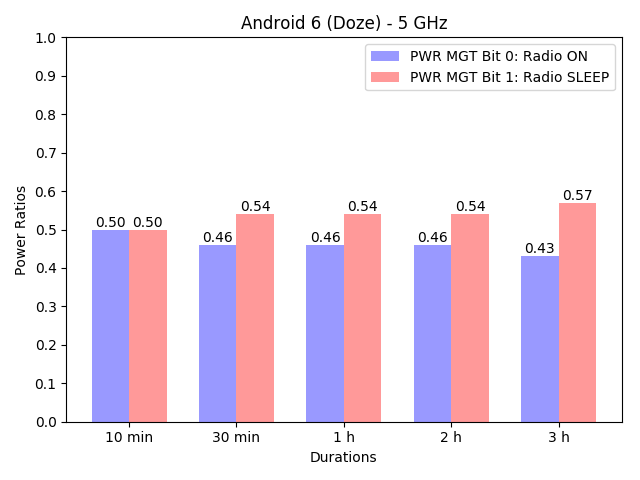
\includegraphics[width=8cm]{04_doze6_pwr_5.png}
              \hfill
              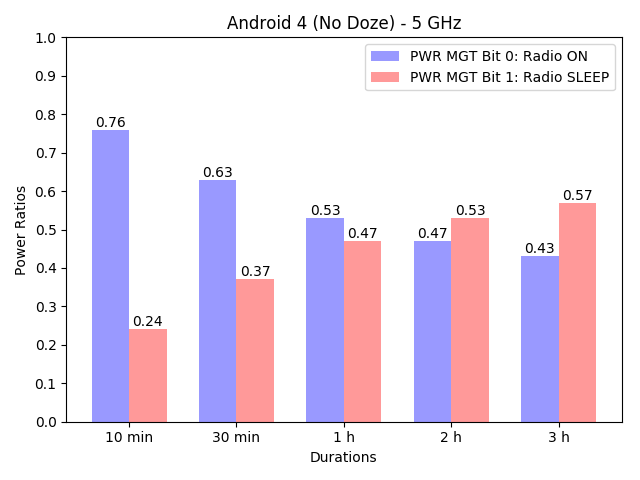
\includegraphics[width=8cm]{05_nodoze4_pwr_5.png}
           }
        \end{figure}

        \begin{figure}[ht]
           \centerline{
              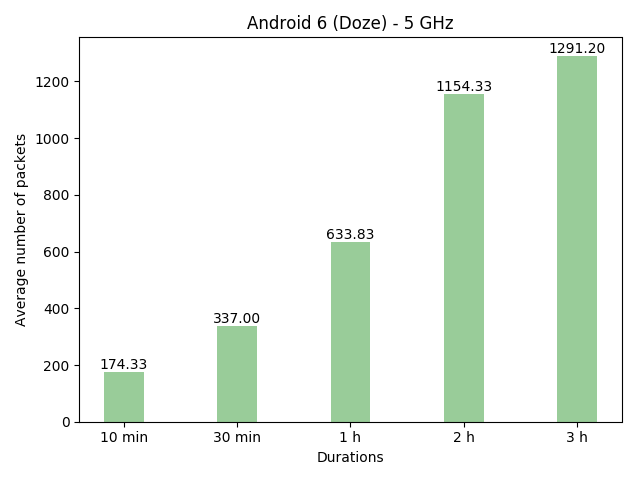
\includegraphics[width=8cm]{06_doze6_avg_pkt_5.png}
              \hfill
              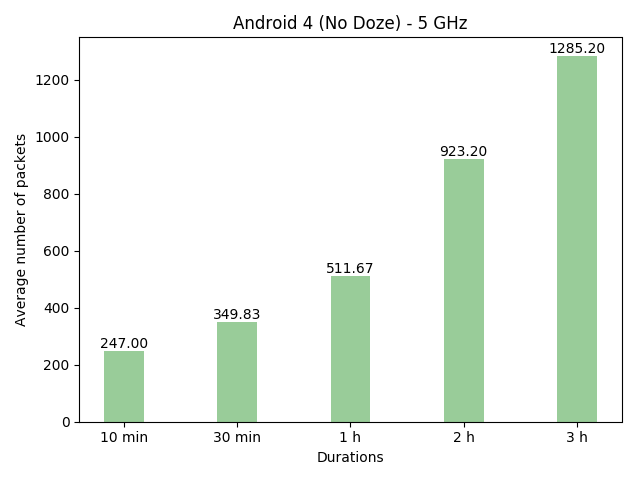
\includegraphics[width=8cm]{07_nodoze4_avg_pkt_5.png}
           }
        \end{figure}
        
        On 5 GHz we still see the same pattern found on 2.4 GHz: power ratios are more stable on Android 6 (Doze) wrt Android 4 (No Doze). 
        Here however the advantage of Dozing seems more evident, in fact on Android 6 on average the 802.11 radio is sleeping 1/2 of the time (PWR MGT bit = 1 $\simeq{0.5}$, PWR MGT bit = 0 $\simeq{0.5}$).
        
        The biggest effects of Dozing can be seen on shorter capture durations (10 min and 30 min) where Android 6 outperforms Android 4 (PWR MGT bit = 1 $\simeq{0.5}$ vs PWR MGT bit = 1 $\simeq{0.3}$), even though Android 4 gradually improves. When reaching 2h and 3h durations the power ratios are the same with and without the usage of Doze. We think that Android 4, even without Doze, has some power management features to save energy on 802.11 after some hours.
        
        In this scenario the average number of packets sent is similar between Android 6 and Android 4 and much less wrt the 2.4 GHz case. We think this happens because 5 GHz consumes more power wrt 2.4 GHz, so to save energy less packets are sent in general.
    
	\section{Conclusions}
	
	From the results of our experiments we can say that Doze positively influences 802.11 power saving functionalities on Android 6 wrt what happens on Android 4 without it. In general, it activates very soon and it is immediately effective. The importance of Doze on 802.11 power saving is further demonstrated by the fact that after Android 6.0, new and improved versions of Doze have been proposed with Android N and Android O.
	
\end{document}
